% プロジェクト学習中間報告書書式テンプレート ver.1.0 (iso-2022-jp)

% 両面印刷する場合は `openany' を削除する
\documentclass[openany,11pt,papersize]{jsbook}



% 報告書提出用スタイルファイル
\usepackage[final]{funpro}%最終報告書
%\usepackage[middle]{funpro}%中間報告書
\usepackage{listings}

% 画像ファイル (EPS, EPDF, PNG) を読み込むために
\usepackage[dvipdfmx]{graphicx,color}

% ここから -->
\usepackage{calc,ifthen}
\newcounter{hoge}
\newcommand{\fake}[1]{\whiledo{\thehoge<70}{#1\stepcounter{hoge}}%
  \setcounter{hoge}{0}}
% <-- ここまで 削除してもよい

% 年度の指定
\thisYear{2015}

% プロジェクト名
\jProjectName{フィールドから創る地域・社会のためのスウィフトなアプリ開発}

% [簡易版のプロジェクト名]{正式なプロジェクト名}
% 欧文のプロジェクト名が極端に長い(2行を超える)場合は、短い記述を
% 任意引数として渡す。
%\eProjectName[Making Delicious curry]{How to make delicious curry of Hakodate}
\eProjectName{``Swift'' Application Development Based on Field Research}


% <プロジェクト番号>-<グループ名>
\ProjectNumber{3-A}

% グループ名
\jGroupName{観光系グループ}
\eGroupName{Tourism Group}

% プロジェクトリーダ
\ProjectLeader{1013220}{新保遥平}{Yohei~Shinpo}

% グループリーダ
\GroupLeader  {1013068}{岩見建汰}{Kenta~Iwami}

% メンバー数
\SumOfMembers{5}
% グループメンバ
\GroupMember  {1}{1013001}{池田俊輝}{Toshiki~Ikeda}
\GroupMember  {2}{1013068}{岩見建汰}{Kenta~Iwami}
\GroupMember  {3}{1013167}{山川拓也}{Takuya~Yamakawa}
\GroupMember  {4}{1013224}{細川椋太}{Ryota~Hosokawa}
\GroupMember  {5}{1013228}{横山翔栄}{Shoei~Yokoyama}

% 指導教員
\jadvisor{伊藤恵,奥野拓,原田泰,木塚あゆみ,南部美砂子}
% 複数人数いる場合はカンマ(,)で区切る。カンマの前後に空白は入れない。
\eadvisor{Kei~Itou,Taku~Okuno,Yasushi~Harada,Ayumi~Kizuka,Misako~Nambu}

% 論文提出日
\jdate{2016年1月20日}
\edate{January~20, 2016}

\begin{document}
%
% 表紙
\maketitle

%前付け
\frontmatter

\input abstract.tex

\tableofcontents% 目次

\mainmatter% 本文のはじまり

\chapter{背景}
\input background.tex

\chapter{到達目標}
\input goal.tex

\chapter{プロジェクトの進め方}
\input project_procedure.tex

\chapter{開発準備}
\input develop_preparation.tex

\chapter{開発プロセス}
\input develop_process1.tex
\input develop_process2.tex
\input develop_process3.tex
\input develop_process4.tex

\chapter{キーコ紀行について}
\section{キーコ紀行の概要}
\input kiko_abstract.tex
\section{「観光する」機能}
\input kiko_cardlist.tex
\input kiko_map.tex
\input kiko_takephoto.tex
\input kiko_textedit.tex
\section{「振り返る」機能}
\input kiko_album.tex
\section{「印刷する」機能}
\input kiko_print.tex
\section{リーフレットについて}
\input kiko_leaflet.tex

\chapter{使用技術}
\input tech_database.tex
\input tech_cardlist.tex
\input tech_map.tex
\input tech_camera.tex
\input tech_album.tex
\input tech_print.tex

\chapter{今後の課題と展望}
\input release.tex
\input connection.tex

\chapter{学び}
\input learned_infoshare.tex
\input learned_planmanagement.tex
\input learned_version_management.tex
\input learned_poster.tex

\chapter{到達目標に対する評価}
\input achievement.tex

\chapter{まとめ}
\input summary.tex

% 以降、付録(付属資料)であることを示す
\begin{appendix}
\chapter{その他新規習得技術}
\section{WebAPI}
アプリケーションの作成にあたり、天気の情報を取得するためにWebAPIを利用した。これはHTTPなどのWeb技術を用いてプログラムの提供する機能を利用するためのサービスであり、有償のものも含め多くの種類が公開されている。本プロジェクトの成果物には``OpenWeatherMap''\footnote{http://openweathermap.org/}を利用しており、このAPIから返されるJSON形式のデータを処理することで、天気情報を表示している。WebAPIの優れている点は、インターネットに接続された環境であればどこからでも利用できるという点である。前述の通り、WebAPIはHTTPなどのWeb技術を用いたサービスである。このため、特殊な機器やシステムを一切使用することなく、多くの機器で普遍的に利用することができる。
\bunseki{横山翔栄}

\chapter{活用した講義}
 報告書の参考文献を明示するために、科学技術リテラシーで学んだ参考文献の書き方の知識を用いた。、また、中間発表で用いたポスターを作成するにあたって、情報表現基礎や情報デザインの講義で得た知識や経験を用いた。見やすく分かりやすいポスターを作るために、できる限り文字を図にして置き換え、図解によって主要を伝えるという点を意識した。また、全体の印象を整えるため各要素の位置を他の要素にそろえた。プロジェクトを進めていくうえでアプリの開発形態を見直すとき、ソフトウェア設計論で学んだウォーターフォールモデルとアジャイル開発手法の考え方を参考にした。本プロジェクトはアジャイル開発手法であり、ウォーターフォールモデルのような1つ1つの段階を固めてから次の段階に進むということはせず、開発を迅速に行いレビューを受け、再び開発をしていくものであるということを常に意識することが重要だと学んだ。アプリはどのような機能を持っているか、ユーザはどのようにアプリを使うのかを明示してそれを設計するためにソフトウェア設計論のユースケース図とアクティビティ図の書き方を参考にした。以下が作成した図である。

\bunseki{山川拓也}

    \begin{figure}{}
        \begin{center}
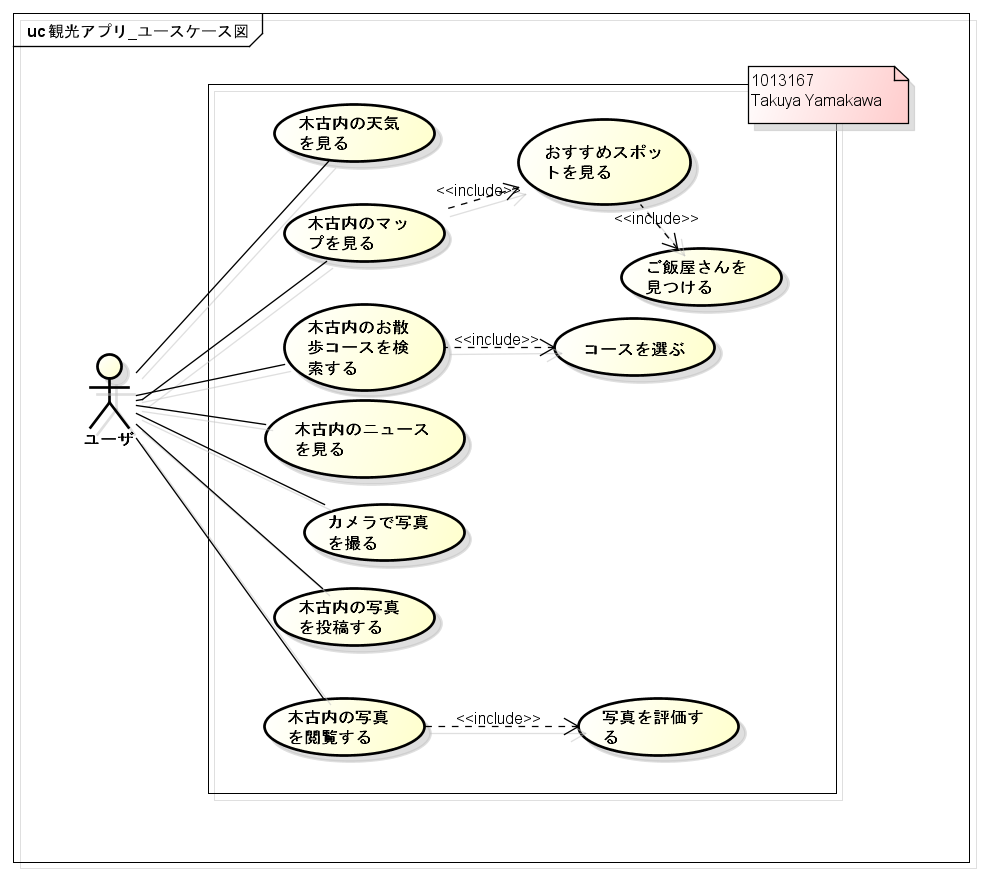
\includegraphics[width=14cm, bb=0 0 520 388]{project_usecase2.png}
        \end{center}
         \caption{ユースケース図}
 \label{fig:one}
      \end{figure}
 

    \begin{figure}{}
        \begin{center}
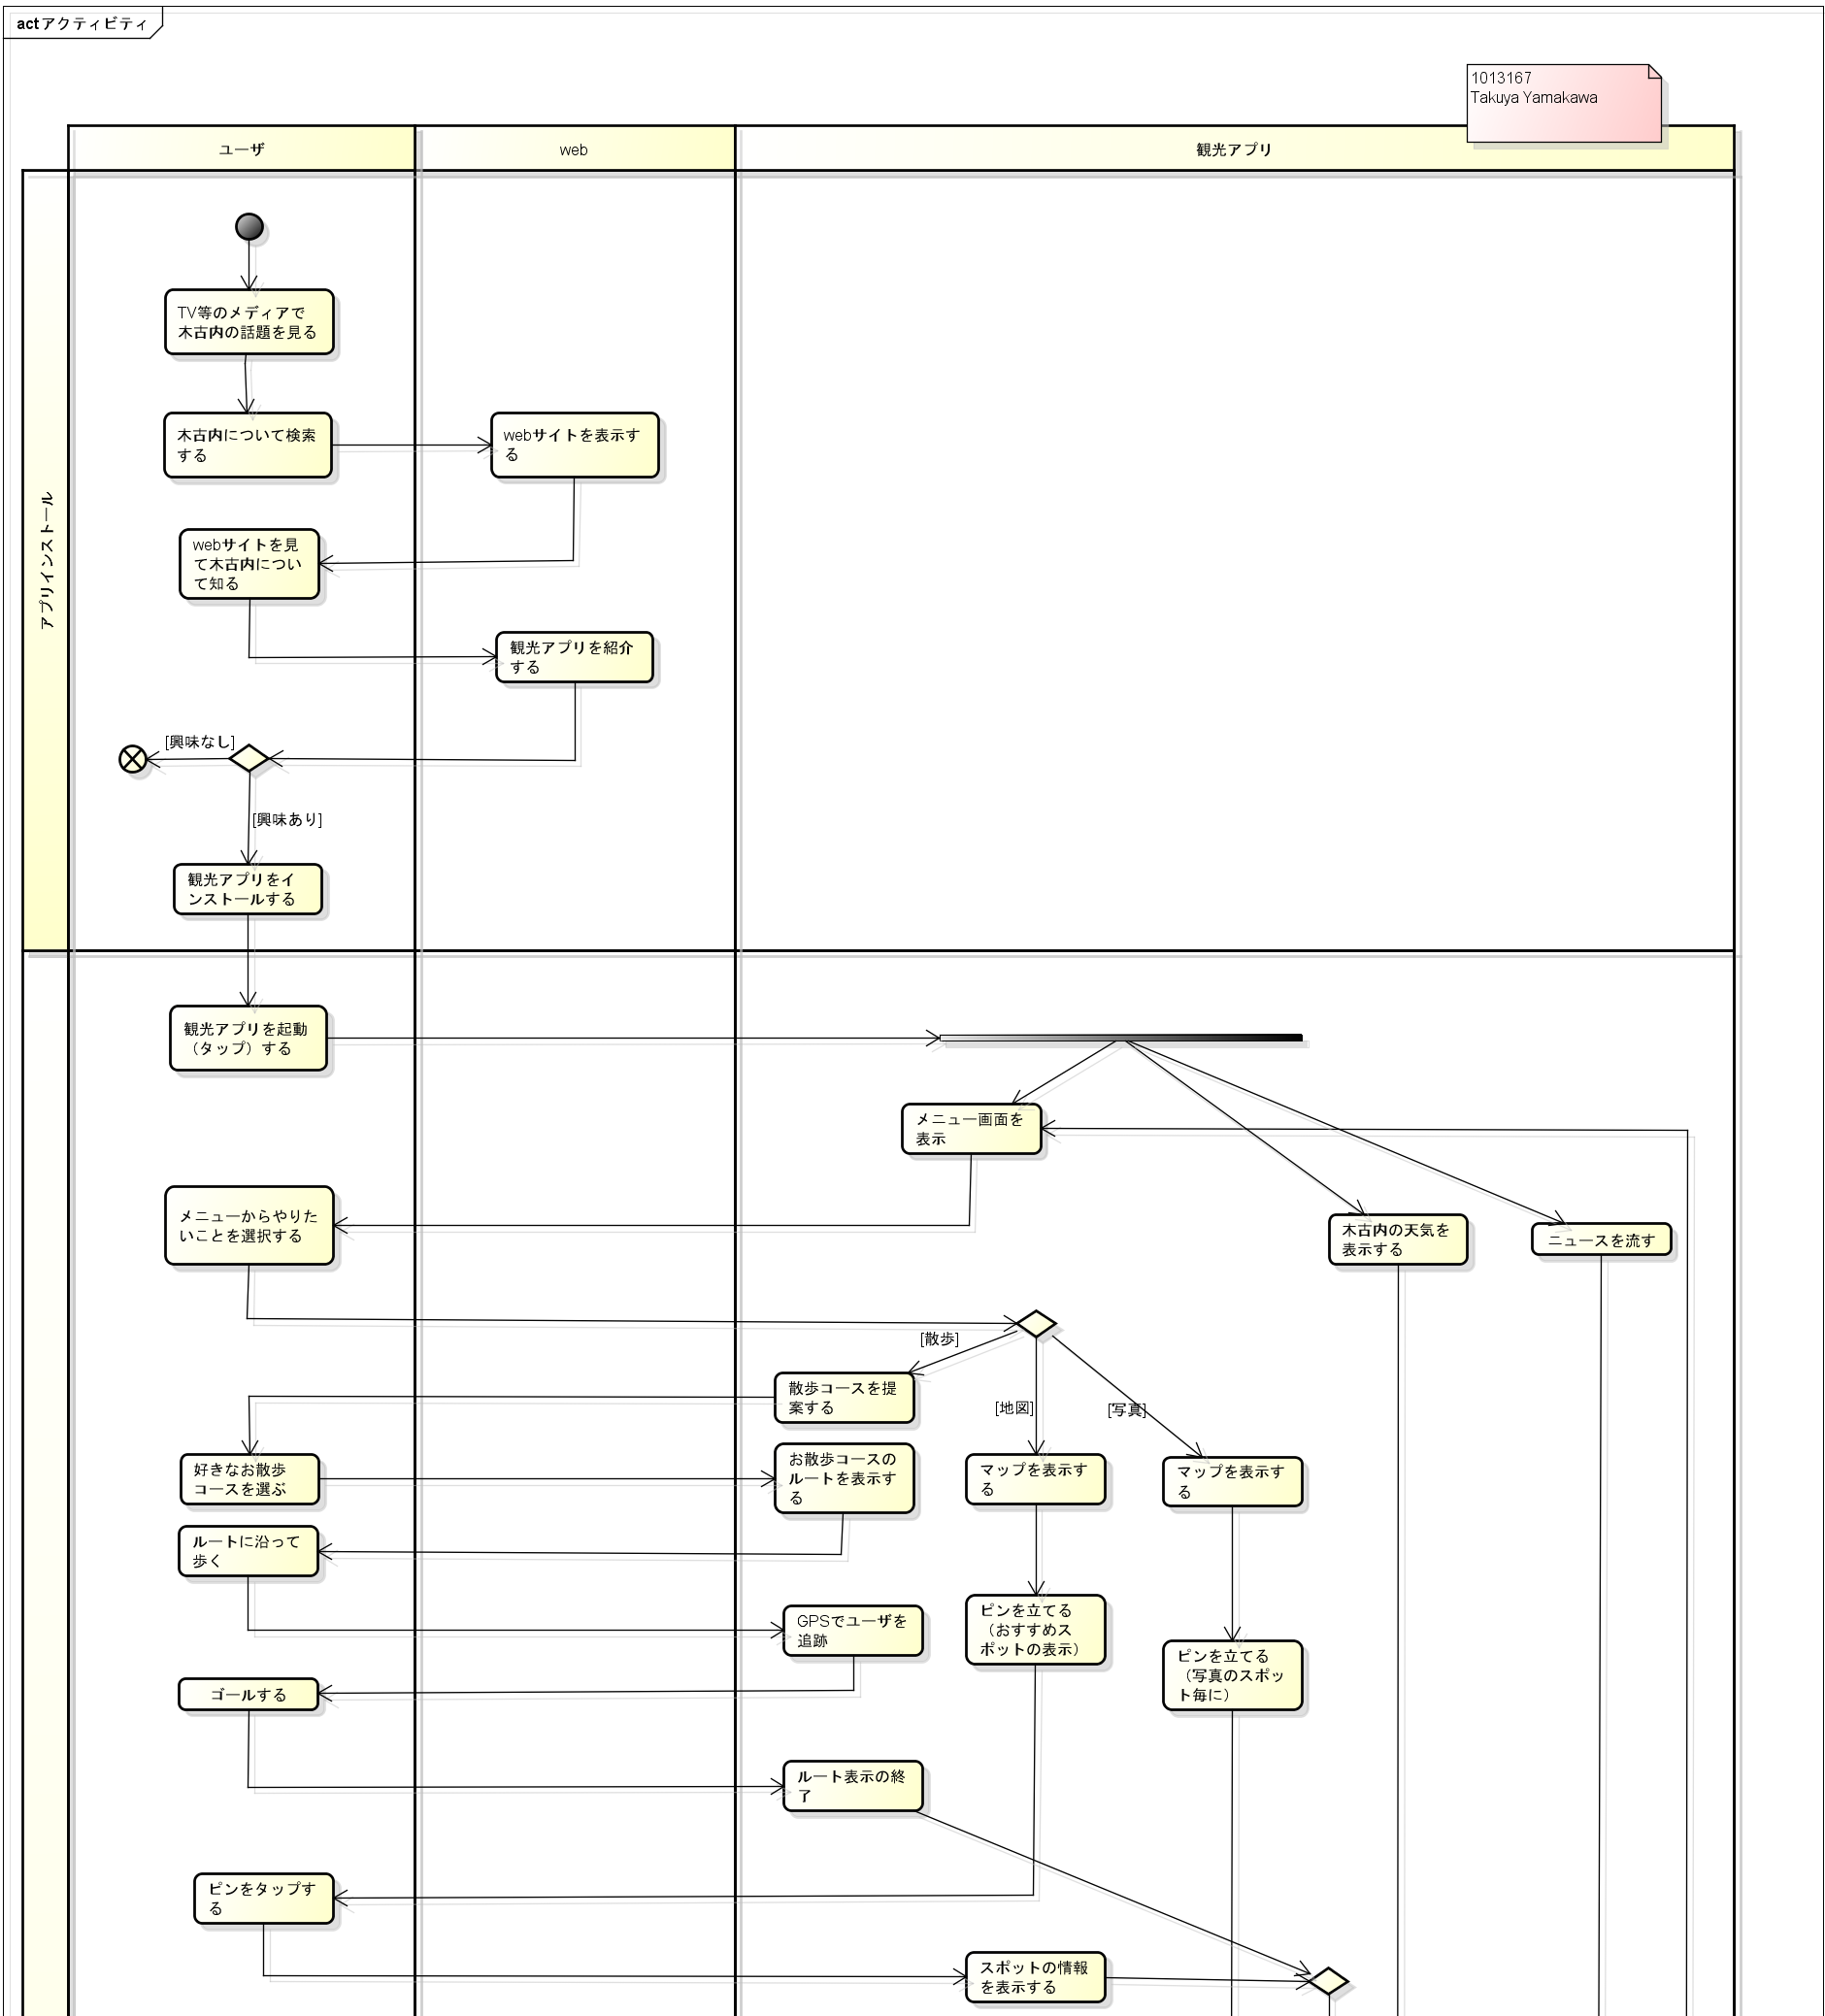
\includegraphics[width=20cm, bb=0 0 1880 2077]{project_activity2.2-1.png}
        \end{center}
 \label{fig:one}
      \end{figure}
      

       \begin{figure}{}
        \begin{center}
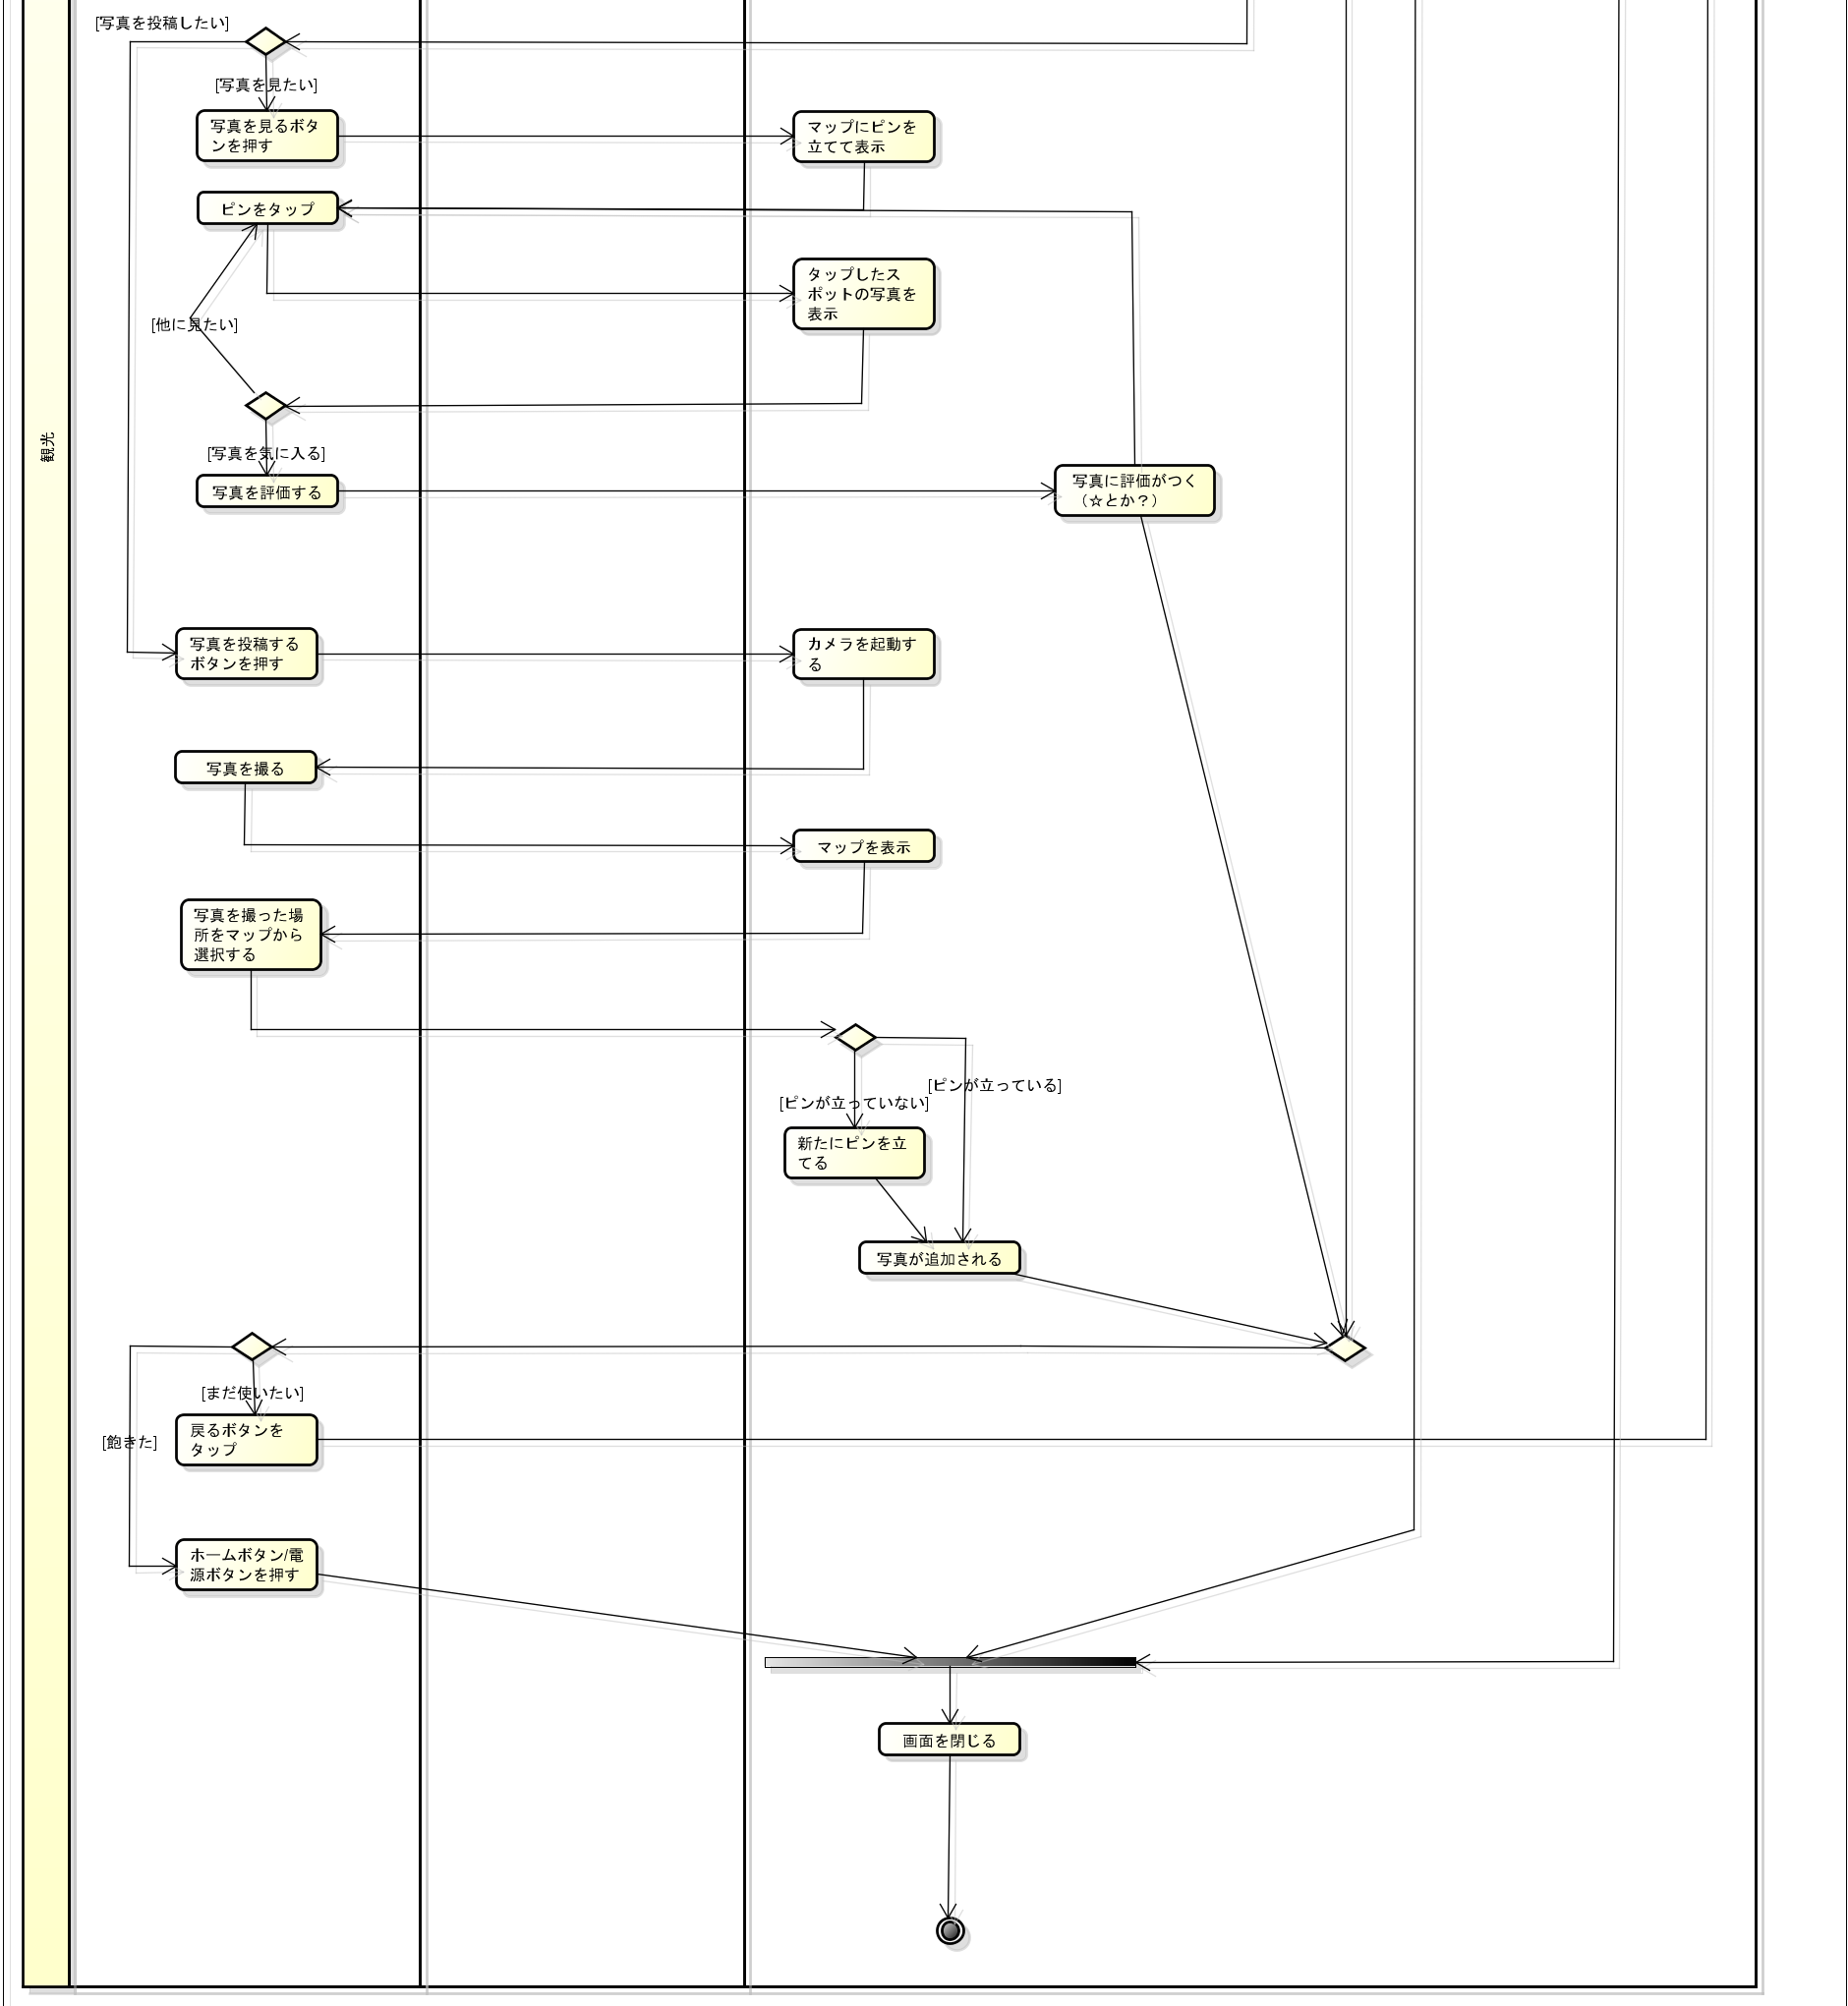
\includegraphics[width=20cm, bb=0 0 1880 2041]{project_activity2.2-2.png}
        \end{center}
                 \caption{アクティビティ図}
 \label{fig:one}
      \end{figure}
      
\chapter{その他成果物}  


\section{Gitマニュアル}
運用ルールとか \\
・プルリクエストは、コメント欄に3人の承認があって初めてマージできるものとする。マージするのは、原則として3人目のコメント者が行う。(あまりにも遅い場合は残りの2人がマージ)\\
・ブランチの切り方については「git-flow」を参照のこと \\ \\
Gitを使った作業の始め方 \\
cd [場所] でどこで作業するか決めて移動する。 \\
git clone [URL] でクローンする。(初回のみ ※1) \\
git branch develop ローカルにdevelopブランチを作る \\
git checkout develop (developブランチにpullするため、移動) \\
git pull origin develop でリモートリポジトリの内容をローカルに反映 \\
git branch で全ブランチ、現在のブランチを確認。 \\
git branch yamakawa で作業ブランチ”yamakawa”を作成。 \\
git checkout yamakawaでブランチの移動。 \\
	git checkout -b yamakawa \\
→(yamakawaブランチを作成して移動)\\
 ファイルを編集・保存 \\
git add [file] \\
git commit -m “commit message” \\
git push origin yamakawa  -$>$  yamakawaブランチをpush \\ \\
※1
もし、pushが403エラーで成功しない場合、cloneするときにgithubユーザ名を付けてみる \\
git clone https://Githubユーザ名@github.com/FUNPBL2015/kan\_practice1.git \\
git pull origin pullしたいリモートブランチ名:ローカルブランチ名 \\ \\
GitHub文化の話… \\
プルリクエスト承認コメントの慣例「LGTM(Looks Good To Me)」 \\
http://d.hatena.ne.jp/keyword/LGTM \\
lgtm.in とかも調べてみる \\ \\
ローカルのmasterがリモートのmasterより遅れているときの解消方法 \\
\$ git graph \\
* (origin/master, origin/HEAD) \\
| \ \\
|  * (HEAD, origin/develop, develop) \\
| / \\
* (master) \\
↑この状態のとき \\
git checkout master \\
git pull origin master \\
で、ローカルのmasterがリモートと同じ位置まで移動する。 \\ \\
リモートリポジトリが壊れた場合、ローカルリポジトリを丸ごとコピーする形で修復を行うこともある。バックアップの意味でも、↑のような状況になっている場合はこの作業を行うこと。 \\ \\
こんな時..... \\
・git status をして、 \\
 Changes not staged for commit: \\
   (use "git add $<$file$>$..." to update what will be committed) \\
   (use "git checkout -- $<$file$>$..." to discard changes in working directory) \\
 modified: kankouApp.xcodeproj/project.xcworkspace/xcuserdata/ \\
\hspace{0.5cm} kouritsuhakodatemiraidaigakukoudoictkosu.xcuserdatad/UserInterfaceState.xcuserstate \\
 と表示されたら、 \\
 git checkout -- $<$赤字をコピペ$>$ すればうまくいける。 \\ \\
・ローカルのブランチを消したい \\
	git branch -d [ブランチ名] \\ \\
・git push origin :test \\
リモートにあるtestブランチを削除できる。 \\ \\
・今いるブランチのローカルでの変更をなかったことにする \\
変更をコミットしてからブランチ切り替えして、と言われた時に使える \\
コンフリクトの時は! \\
エラーメッセージに従って処理  \\


%付録の終わり
\end{appendix}

% 参考文献
\begin{thebibliography}{99}

\bibitem{KIKONAI_HP}
木古内町. 木古内町観光協会. http://kikonai-kankou.net/ (2015/7/22 アクセス)

\bibitem{GITFLOW}
gitflow cheatsheet. danielkummer.github.io. \par
http://danielkummer.github.io/gitflowcheatsheet/index.ja\_JP.html \par
(2016/01/06 アクセス)

\bibitem{TIMEOUTTOKYO}
Time Out Tokyo. 札幌でしかできない50のこと - Time Out Tokyo (タイムアウト東京). \par
http://www.timeout.jp/tokyo/ja/things-to-do/sapporo \par
(2016/01/19アクセス)

\bibitem{FUJI}
富士フィルム株式会社. フジフイルムのフォトブックでフォトアルバムを作成 \par
http://f-photobook.jp/ (2016/01/19アクセス)

\bibitem{TIGAI}
株式会社ルックバイス. 「カタログ」と「パンフレット」と「リーフレット」の違い - 違いが分かる辞典. \par
\url{http://chigai-allguide.com/%E3%82%AB%E3%82%BF%E3%83%AD%E3%82%B0%E3%81%A8%E3%83%91%E3%83%B3%E3%83%95%E3%83%AC%E3%83%83%E3%83%88%E3%81%A8%E3%83%AA%E3%83%BC%E3%83%95%E3%83%AC%E3%83%83%E3%83%88/} 
(2016/01/19アクセス)

\bibitem{REALM}
Realm. Y Combinator. 2015. https://realm.io/jp/. (2016/1/18 アクセス)

\bibitem{CUSTOMCELL}
BigSea. SwiftでCustomCellを作って画像付きリスト表示. \par
http://qiita.com/BigSea/items/9aa35b95e5d4d1dc8a52. (2016/01/07アクセス)

\end{thebibliography}
\end{document}